\chapter{Introduction}\label{ch:introduction}

\section{Outflows from BNS Mergers}
    \label{sec:bns}
    Due to the joint electromagnetic and gravitational wave detection of the
    binary neutron star coalescence known as GW1701817 (see
    \cite{abbott_gw170817_2017}), there has been renewed interest in sGRBs.
    Specifically, the claim that SGRBs have binary neutron star mergers as
    their central engines  (see \cite{narayan_gamma-ray_1992}) gained
    credence because of this detection. There are other aspects of the
    process that are not as clear. Specifically, several aspects of GW170817
    have not been completely explained. The main concerns are as follows
    \cite{lazzati_short_2020}:

    \begin{itemize}

        \item The outflow of GRB170817A was lower in energy, compared to that of
            a typical cosmological SGRB, by a factor of $10^4 - 10^5$, even
            though the event was one of the closest GW events recorded, at a
            distance of $\sim$ 40 Mpc. This could be due to two factors :

            \begin{itemize}

                \item The observer being off-axis with respect to the structured
                    jet.

                \item The internal engine powering this SGRB was intrinsically
                    less energetic, and differs from the one observed in other
                    typical SGRBs.
            \end{itemize}

        \item A clear consensus has not been reached on how the gamma-ray prompt
            emission was produced. The uncertainty partly comes from the fact
            that the various delays involved before the prompt emission is
            observed are not accurately constrained. Models which have been
            considered include :

            \begin{itemize}

                \item The structured outflow model, characterised by functions
                    for the Lorentz factor and the energy per unit solid angle,
                    both of which vary with the angle made with the polar jet
                    axis ($\theta$). This model produces detectable signals even
                    at moderately large off-axis angles.

                \item The shock breakout model, wherein the leading edge of the
                    wind emits the prompt emission as it breaks out of the
                    cocoon of nuclear matter ejected before the jet was
                    launched. This model has been shown to explain the
                    energetics and spectrum of the prompt emission, although it
                    does require a setup in which the wind is fast enough so
                    that it can reach a large enough distance at breakout.

            \end{itemize}

    \end{itemize}

    More light can be shed on these questions by observing more such SGRBs,
    using both the gravitational wave (GW) and electromagnetic (EM) windows.
    However, the possibility of joint detections are slim, due to the fact that
    the EM observations are highly dependent on the viewing angle of the system
    with respect to the observer (due to relativistic beaming), whereas GW
    signal amplitudes depend on the distance to the event
    \cite{saleem_prospects_2020}.\\ Given that this is the case, it is expedient
    to look for constraints on the structure parameters of various models.
    Furthermore, it is useful to develop models which are resilient to
    non-detections, and can produce constraints on the parameters using upper
    limits on the flux/fluence observed by the various EM follow-up satellites,
    such as INTEGRAL, Fermi or Swift.

    As mentioned before, the electromagnetic follow-up of the binary neutron
    star merger event GW170817 helped measure the various time delays between
    the time of the GW signal trigger (which roughly is the merger time itself)
    and the time the gamma-ray signals were picked up. This time delay is
    denoted $\Delta t_{GW-\gamma}$, and was around 1.75 seconds for this event.
    The components which make up this delay are as follows
    \cite{lazzati_short_2020}:

    \begin{itemize}

        \item \textbf{Engine Delay} : this is the delay due to some transition
            mechanism in the central engine which powers the jet (such as a
            metastable, fast spinning neutron star which collapses into a black
            hole when its rotation period increases; this process can take
            years) or due to the need of amplifying the magnetic field to a
            value large enough to launch the jet  (this process is significantly
            faster, taking seconds). This is denoted by $\Delta t_{eng}$.

        \item \textbf{Wind Delay} : this is simply a delay in the launching of a
            non-relativistic wind due to the neutron-rich matter from the
            progenitors being tidally shredded. For this reason, it can be
            \textit{negative} as well, since the tidal shredding can occur
            before the merger itself. This is denoted as $\Delta t_{wind}$.

        \item \textbf{Breakout Delay} : if the wind is ejected before the jet,
            then the latter will have to propagate through the former and this
            happens at a sub-relativistic speed, whereas the GW signal travels
            at a relativistic speed. The delay due to this crossing is the
            breakout delay, and is denoted $\Delta t_{bo}$. During this time,
            jet-wind interactions cause the development of a structured outflow
            that maintains a bright core but also has energetic wings at large
            polar angles.

        \item \textbf{Photospheric Delay} :  once the jet has crossed the wind,
            it still needs to propagate out to the photospheric radius, where
            the outflow becomes transparent and the prompt gamma-ray emission is
            radiated. The delay from the breakout radius to the photospheric
            radius is $\Delta t_{ph}$. This is given as (for GW170817):

            \begin{equation}
                \label{eq:4}
                \Delta t_{ph} \sim \dfrac{R_{ph}}{c \Gamma^2} =
                1.4 \dfrac{R_{ph}}{2 \times 10^{12} \text{ cm}}
                \left( \dfrac{7} {\Gamma} \right)^2 \text{ s}
            \end{equation}

        \item \textbf{Dissipation Delay} : this is a requirement in some models,
            such as the internal shock synchrotron model, wherein the outflow
            needs to travel to the internal shock radius before the bulk energy
            of the flow is dissipated and turned into radiation. The time
            required to get to this point after crossing the photospheric radius
            is the dissipation delay, denoted $\Delta t_{\gamma}$

    \end{itemize}


    Several attempts to constrain the various time delay components have been
    made. However, except for relative comparisons, no conclusions have been
    arrived upon.  For example, one can only say that the photospheric delay is
    the major component out of all the delays, and that wind delay (if non-zero)
    has to be lesser than the jet delay, so that the jet catches up to the wind
    and the jet-wind interaction generates the structured outflow. The figure
    below summarises these delays in the broader context.

    \begin{figure}[H]
        \label{fig:jet_delay}
        \centering
        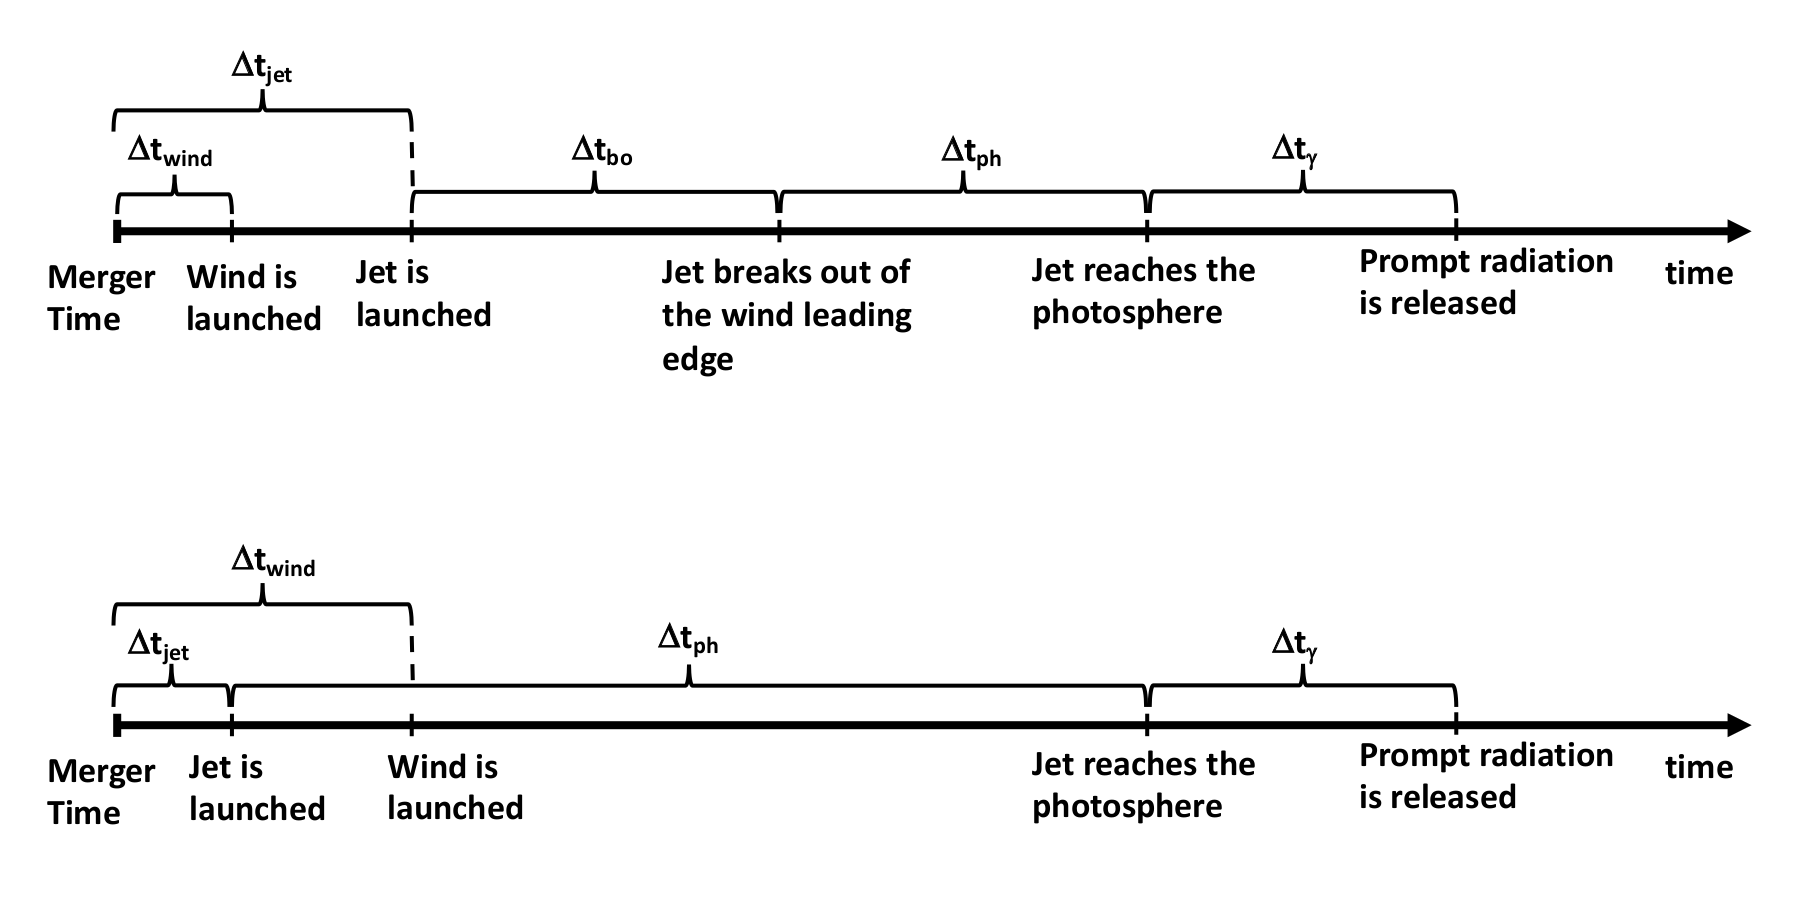
\includegraphics[width=12cm]{jet_delay}
        \caption[Relative Positions of Jet Delays]{
                    Two possible scenarios for the relative positioning of the
                    delays in time, which contribute to $\Delta t_{GW-\gamma}$.
                    Owing to the requirement of a structure outflow, GW170817
                    possibly follows the top timeline. The relative
                    contributions of the various delays are debated, but it is
                    agreed that $\Delta t_{wind} < \Delta t_{jet} \ll 1$ s,
                    $\Delta t_{bo} \ll 1$ s, $\Delta t_{\gamma} \sim 0$ and
                    $\Delta t_{ph} \sim \Delta t_{GW-\gamma}$.
             }
    \end{figure}

    Due to the uncertainties in the delay terms, several models for the jet can
    explain the energetics and observed structure. Numerical simulations are
    also not unequivocal about their favouring of one model over the other (see
    \cite{shibata_merger_2019}). Some models try to explain the apparent
    structure of the jet, that is the observables seen by a particular observer
    at a particular viewing angle. Other models are used to explain the
    \textit{intrinsic} structure, such as the polar angle variation of the bulk
    Lorentz factor and the energy across the solid angle, in the jet co-moving
    frame (see \cite{salafia_structure_2015} for a detailed discussion of the
    differences between the two structures). Some of these are given below (see
    also Figs. \ref{fig:tophat} and \ref{fig:jet_models}):

    \begin{itemize}

        \item Top-hat : This model, as used in \cite{saleem_energetics_2020},
            assumes that the bulk Lorentz and energy functions drop to zero
            beyond some cutoff angle, $\theta_j$. Below this threshold, the
            functions are at their respective on-axis values.

       \item Gaussian : This model is widely used, in some contexts to explain
           the apparent jet structure (by \cite{hayes_comparing_2020}), and in
           others the intrinsic jet structure (by
           \cite{saleem_energetics_2020}). The former is simply given by
           $y_{GJ}(\theta) = e^{- \frac{1}{2} \left(
           \frac{\theta}{\theta_{\sigma}} \right)^2}$, since the authors
           consider only the apparent jet structure, as explained above and
           $\theta_\sigma$ is a structure parameter which is inferred by the
           authors' Bayesian inference.\\
           In the latter, as the authors consider the intrinsic jet structure,
           they assume that $\Gamma \beta (\theta)
           = \Gamma_0 \beta_0 \exp\left(- \theta^2 / 2\theta_c^2\right)$ and
           that $\epsilon (\theta) \propto \exp(- \theta^2 /
           \theta_c^2)$\footnote{This is the normalised energy profile function.
           The normalisation constant is estimated by the condition $2\pi \int
           d(\cos \theta) \epsilon(\theta) = E_{tot., \gamma}$, where $E_{tot.,
           \gamma}$ is the total energy in gamma-rays.}, and derive the observed
           properties (see below).

        \item Power Law : This model is used by \cite{hayes_comparing_2020} to
            explain the apparent structure of the jet, assuming that any
            variation in the energy is simply because of relativistic beaming
            and the jet being viewed off-axis. It is given using the shape
            function $y(\theta)$ (which is multiplied with the on-axis isotropic
            equivalent energy $E_{iso, 0}$ to give
            $E_{iso}(\theta)$\footnote{Using the equation $E_{iso}(\theta_v) =
            E_{iso, 0} \cdot y(\theta_v)$}):

                \begin{equation}
                    \label{eq:5}
                    y(\theta) = \begin{cases}
                                    1,
                                        & 0 \leq \theta \leq \theta_c, \\
                                    (\theta/\theta_c)^{-2},
                                        & \theta_c < \theta \leq \theta, \\
                                    0,
                                        & \theta_j < \theta
                                \end{cases}
                \end{equation}
                Here $\theta_c$ and $\theta_j$ are simply structure parameters,
                inferred using Bayesian methods.

    \end{itemize}

    \begin{figure}[H]
        \centering
        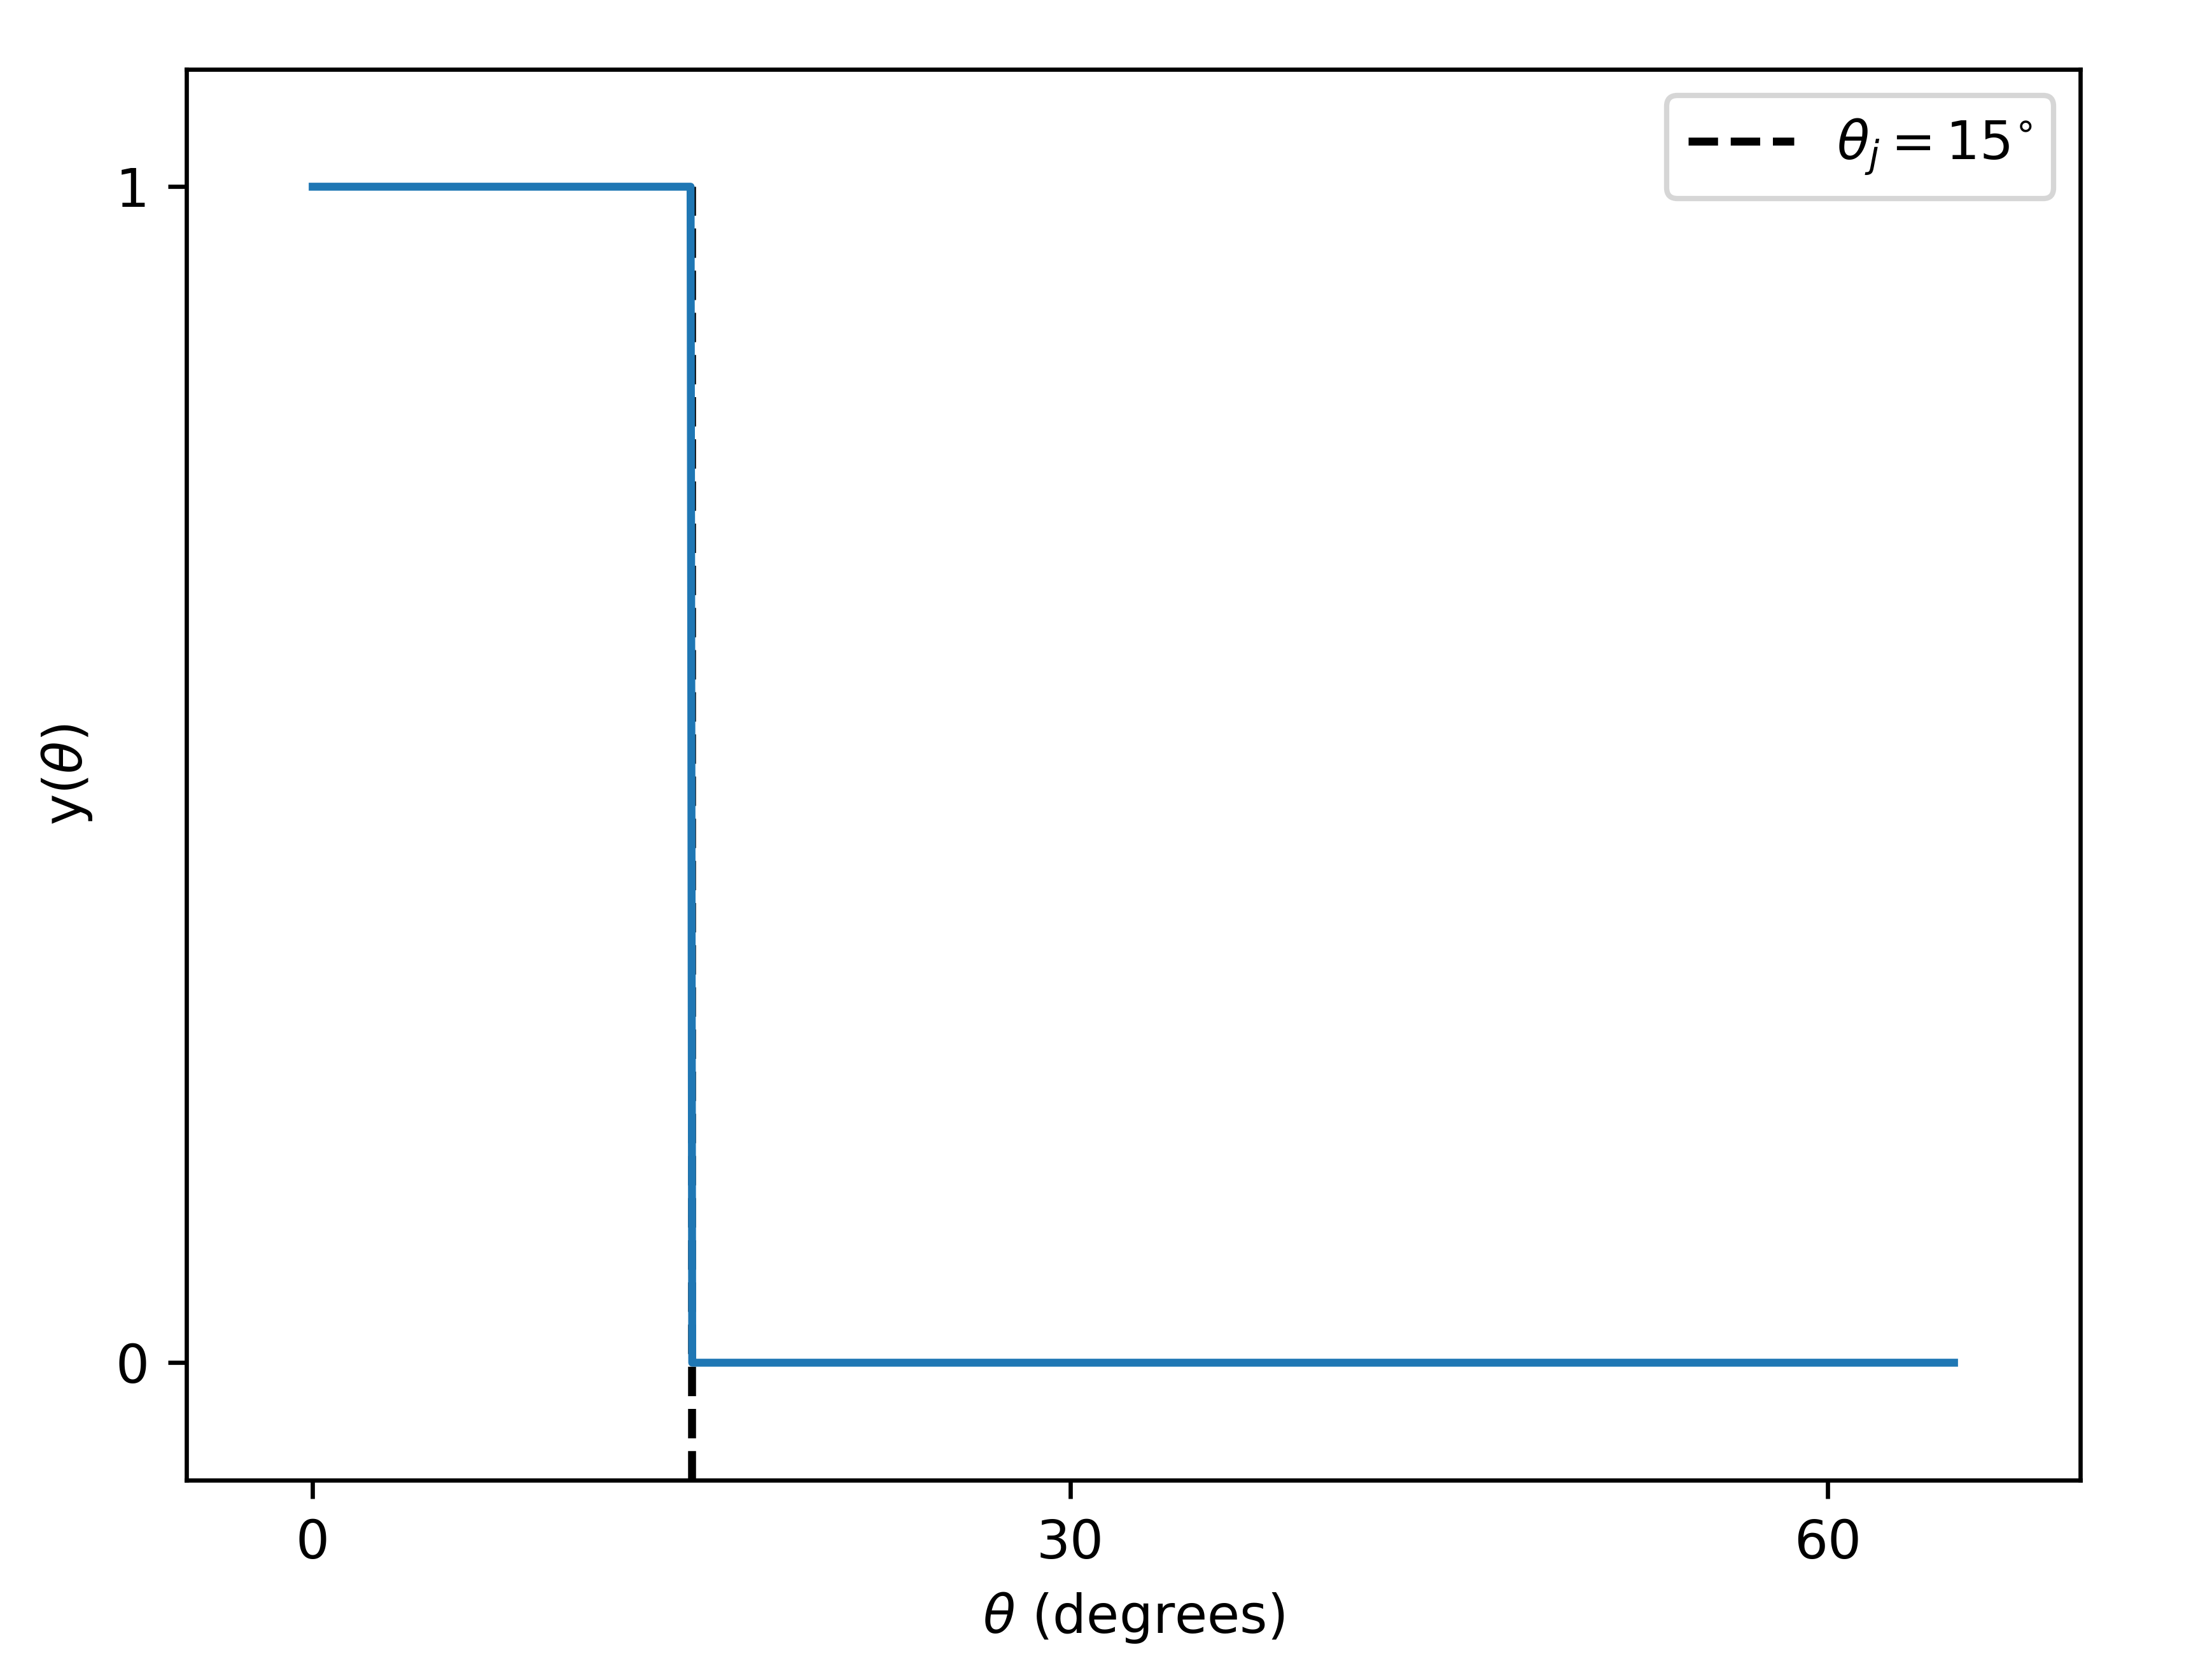
\includegraphics[width=9cm]{tophat}
        \caption[Tophat jet structure model]{
                    Functional form of the tophat jet structure model, as considered in
                    \cite{saleem_energetics_2020}. The dashed line denotes the jet angle
                    $\theta_j = 15^{\circ}$.
             }
        \label{fig:tophat}
    \end{figure}

    \begin{figure}[H]
        \centering
        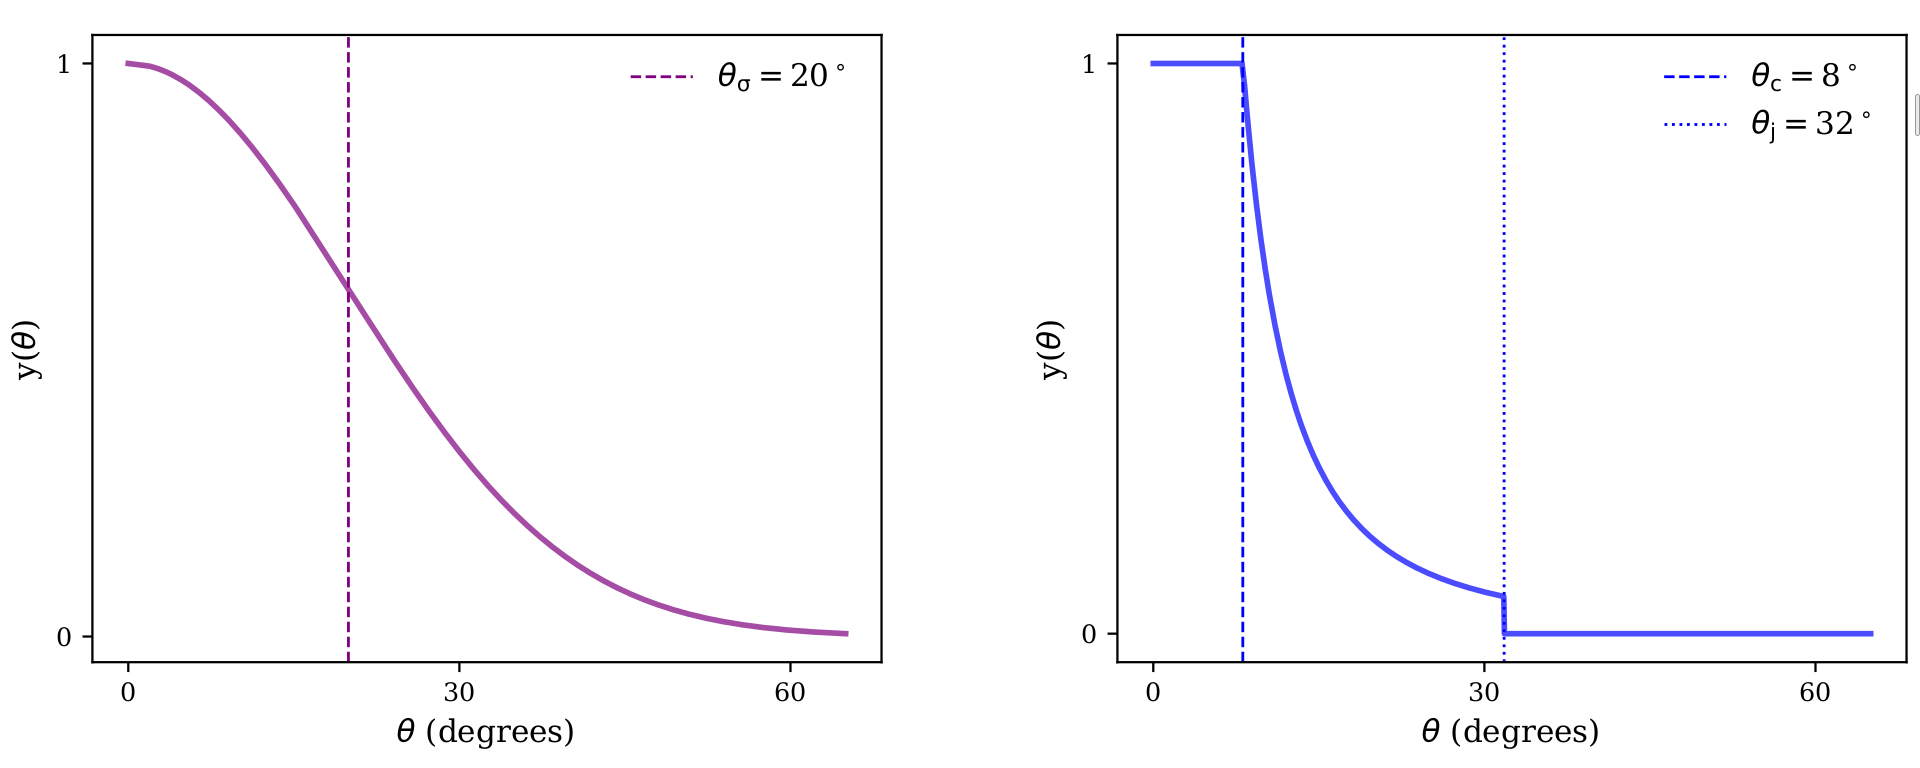
\includegraphics[width=\textwidth]{jet_models}
        \caption[Jet structures as in \cite{hayes_comparing_2020}]{
                    Functional forms of the jet structure models, as considered by
                    \cite{hayes_comparing_2020}. (Left) The gaussian jet structure with
                    a width $\theta_{\sigma} = 20^{\circ}$, also marked by the dashed
                    line. (Right) The power-law structure with a core angle $\theta_c =
                    8^\circ$ and a jet angle $\theta_j = 32^\circ$.
             }
        \label{fig:jet_models}
    \end{figure}

    In order to start off with an intrinsic structure and calculate the observed
    structure, following \cite{granot_off-axis_2002}, we start off by
    considering the emission profile of a point source moving at some angle with
    the observer, essentially rendering this scenario off-axis. This will affect
    the prompt jet emission, as well as the initial afterglow, and so warrants
    careful analysis.  Now, let the initial jet opening angle be $\theta_0$ and
    let the observer be at an angle $\theta_{obs}$. In general, for a point
    source moving at any angle $\theta$ with respect to the observer, the
    observed flux is given by :

    \begin{equation}
        \label{eq:1}
        F_{\nu} =
           \dfrac{L^{\prime}_{\nu^{\prime}}}{4 \pi d_L^2}
           \left( \dfrac{\nu}{\nu^\prime}\right)^3
                =
            \dfrac{1 + z}{4 \pi d_L^2}
            \dfrac{L^{\prime}_{\nu^{\prime}}}{\gamma^3 (1 - \beta \cos \theta)^3}
    \end{equation}

    Here, $L^{\prime}_{\nu^{\prime}}$ and $\nu^{\prime}$ are the jet comoving
    frame spectral luminosity and frequency, $d_L$ is the luminosity distance,
    $\gamma = (1 - \beta^2)^{-1/2}$ is the jet Lorentz factor. If $t$ and $\nu$
    are the observed time and frequency  for an observer at $\theta$, and $t_0$
    and $\nu_0$ are those for an observer on the axis, then:

    \begin{equation}
        \label{eq:2}
        \dfrac{t_0}{t} =
            \dfrac{\nu}{\nu_0}
                       =
            \dfrac{(1 - \beta)}{(1 - \beta \cos \theta)}
            \equiv a
            \approx \dfrac{1}{(1 + \gamma^2 \theta^2)}
    \end{equation}

    And finally putting Eq. \ref{eq:2} into Eq. \ref{eq:1} and expanding using a
    Taylor series approximation upto the leading order:

    \begin{equation}
        \label{eq:3}
        F_{\nu}(\theta_{obs}, t) =
            a^3
            F_{\nu/a}(0, at)
    \end{equation}

    This gives us a handle on how to relate observed off-axis quantities to the
    on-axis ones. Furthermore, this enables us to go from an intrinsic structure
    to an observed one, which is what was required.

\section{Outflows from NSBH Mergers}

    The difference in this pathway to sGRBs, compared to the case of BNS mergers, is
    that though there is theoretical and simulational support for the launching of sGRB
    jets from the merger of a neutron star and a black hole of appropriate mass (see for
    example \textbf{citations}), there has not been strong evidence from the
    observational side of things. In the first half of the third observing run of the
    LVC (also known as O3a), there have been several triggers which have been reportedly
    confident NSBH triggers. However, there were no counterpart EM signals picked up,
    which decreases the credibility of NSBH mergers as the progenitors of sGRBs.\\

    The electromagnetic component from NSBH mergers, is largely decided based on the
    amount of mass left post-merger, outside the horizon of the black hole. This decides
    how much matter participates in the subsequent processes, which may be the rapid
    neutron-capture process which gives rise to the kilonova signal or the magnetic
    field amplification via magneto-rotational instability which leads to a sGRB jet.\\

    Qualitatively, for a binary where the neutron star is treated as a test mass and the
    black hole's spin is aligned with the orbital angular momentum of the binary, the
    innermost-stable circular orbit radius $r_{ISCO}$ scales as $r_{ISCO} \sim
    f(\chi_{BH}) G M_{BH}/c^2$ (where f is a function ranging from 1 to 9, decreasing
    for increasing (prograde) spins; see \cite{bardeen_1972}) and the radius at which
    the tidal disruption of the neutron star starts, $r_{dis}$ scales as $r_{dis} \sim k
    (M_{BH/M_{BNS}})^{1/3} R_{NS}$ (where k is a constant with a dependence on the black
    hole spin and the equation of state). Only requiring that $r_{dis} \gtrsim
    r_{ISCO}$, as a rough requirement for disruption to occur before the neutron star
    plunges into the black hole, leads to the conclusion that (a.) low-mass black holes
    (b.) larger NS radii (c.) higher prograde black hole spins favour disruption. This
    is seen as well from Fig. \ref{fig:nsbh_disruption_condition}. However, the actual
    quantitative results need to be simulated such the effect of the various components
    in the problem are correctly taken into account. As seen from carrying these
    simulations out, the matter left over post-merger heavily depends on (for a summary,
    see Fig. \ref{fig:rest_mass_fraction}):

    \begin{itemize}

        \item The mass ratio of the system. This is defined as $q = M_{BH} / M_{NS}$ so
            that $q > 1$ always. Fully general relativistic, magnetohydrodynamic
            simulations (such as \cite{ruiz_2020}) show that in cases where the  mass
            ratio is 3:1, regardless of the neutron spin, a collimated outflow is
            observed, whereas the same is not realised in cases where the mass ratio is
            5:1 or higher.
        \item The spin of the components of the system. In geometrized units (where $G =
            c = 1$), these are prescribed in terms of $a_{BH} / M_{BH}$ or $a_{NS} /
            M_{NS}$, and whether these two spins align (prograde) or are anti-aligned
            (retrograde) decides whether the neutron star would be tidally disrupted,
            and hence participate in the processes mentioned previously, or not. Via
            simulations, it is seen that the more the prograde spin of the neutron star,
            the farther out the neutron star is tidally disrupted, albeit this is only
            observed for the case of q = 3:1 (comparing say, Figs. \ref{fig:nsbh_jet}
            and \ref{fig:nsbh_5to1}). Also, this leads to long tidal tails, which
            produces a baryon-loaded environment and thus the magnetic field of the
            tidally disrupted matter must overcome the baryon ram pressure to launch the
            jet. This process hence delays the launching of the jet.
    \end{itemize}

    Aside from the sGRB jet, which requires magnetic field amplification (via MRI) as
    well as thermal pair production (from the disk remnant) followed by the
    Blandford-Znajek process, there is a possibility that NSBH mergers can produce
    kilonovae signatures. For this, the dynamically ejected mass has to be between
    $10^{-4.5} - 10^{-2} (M_{NS}/1.4 M_{\odot}) M_{\odot}$ (see \cite{ruiz_2020} for
    more details), and this will lead to kilonovae potentially detectable by the Large
    Synoptic Survey Telescope (LSST).

    \begin{figure}[H]
        \centering
        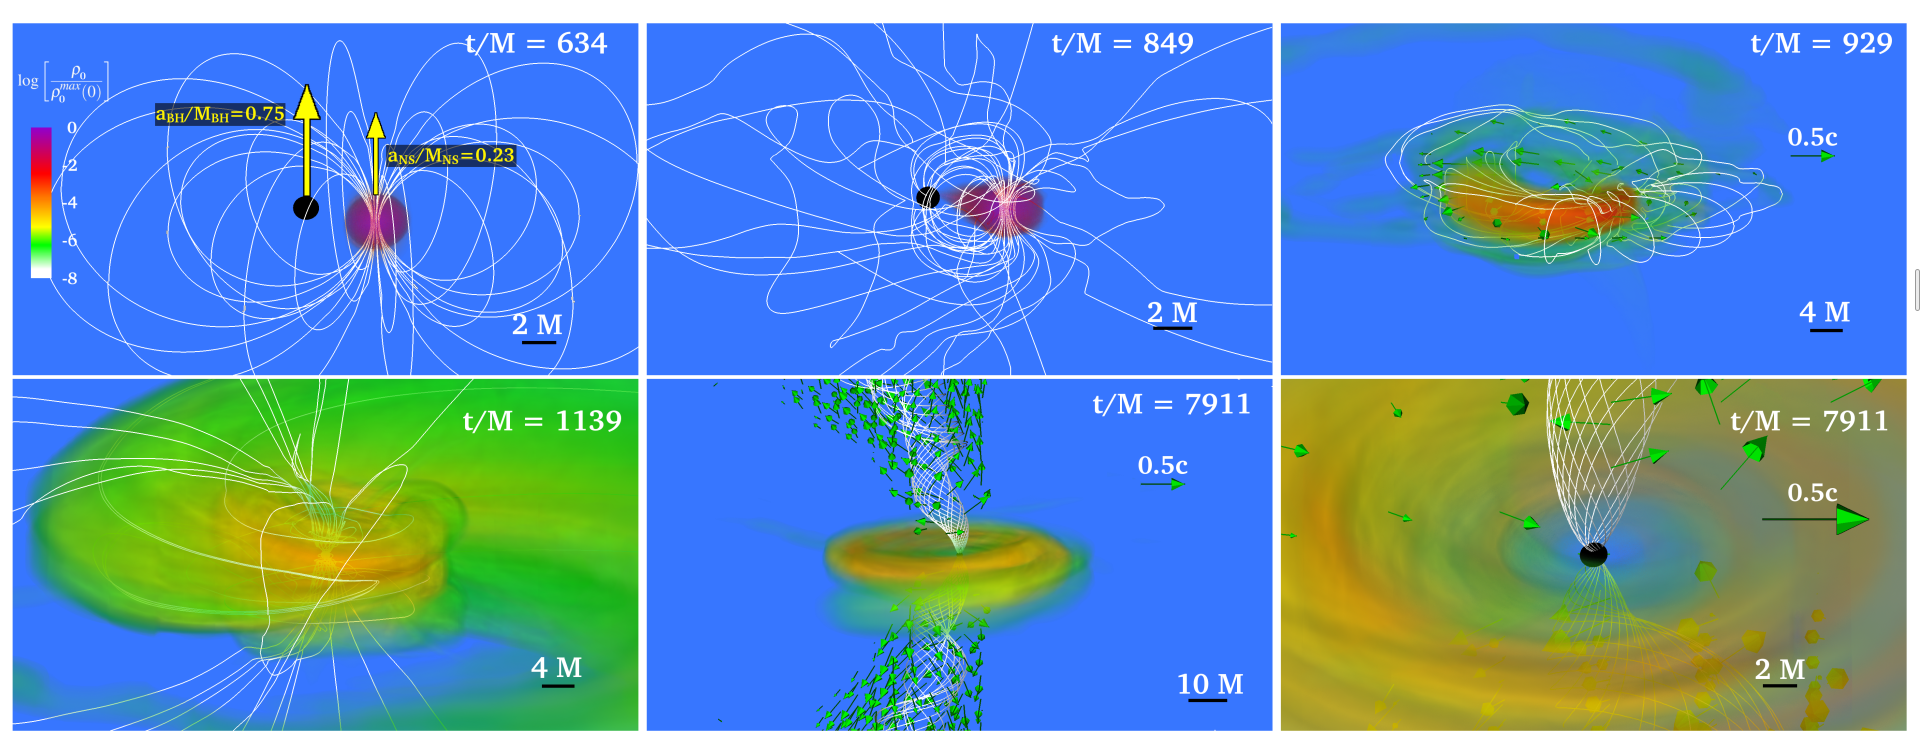
\includegraphics[width=\textwidth]{nsbh_jet}
        \caption[Tidal disruption of a NS in a 3:1 NSBH binary]{
                    Volume rendering of the rest mass density ($\rho_0$) (in log scale),
                    normalized to the NS maximum value $\rho_0 = 8.92 \times 10^{14}
                    (1.4 M_{\odot}/M_{NS})^2 \text{ g/cm}^3$, for particular times for a
                    magnetized neutron star, with q = 3:1 and a prograde NS spin of
                    0.23.  Top three panels highlight the inspiral and the tidal
                    disruption, whereas the bottom three panels highlight the appearance
                    of the magnetically-driven jet. White lines denote the magnetic
                    field, arrows denote the fluid velocity and the BH's apparent
                    horizon is the black sphere. Here M = $2.5 \times 10^{-2}
                    (M_{NS}/M_{1.4M_{\odot}}) \text{ ms} = 7.58
                    (M_{NS}/M_{1.4M_{\odot}}) \text{ km}$ (in geometrized units). From
                    \cite{ruiz_2020}.
             }
        \label{fig:nsbh_jet}
    \end{figure}

    \begin{figure}[H]
        \centering
        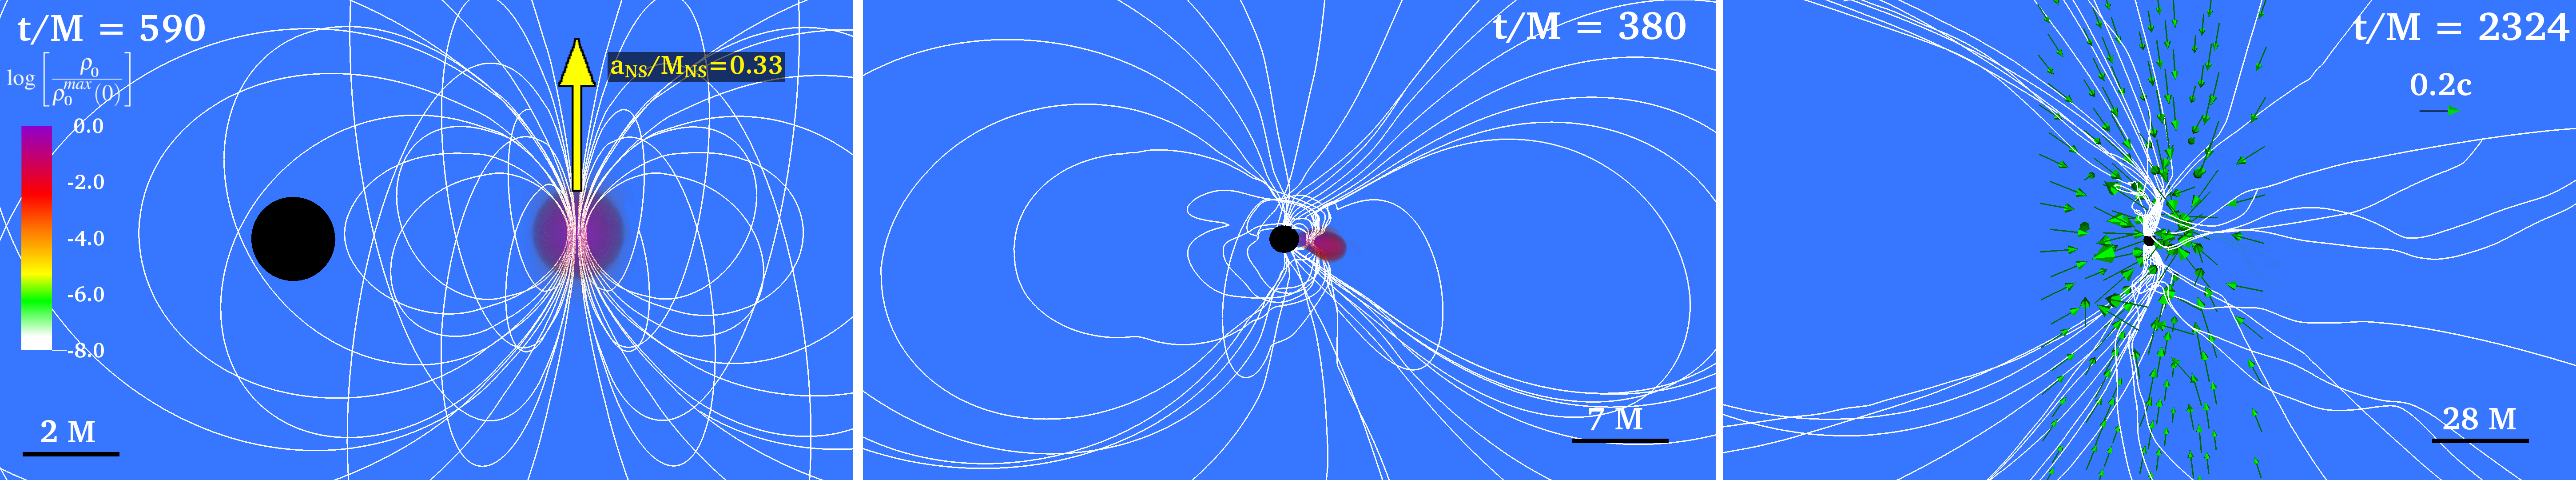
\includegraphics[width=\textwidth]{nsbh_5to1}
        \caption[Tidal disruption of a NS in a 5:1 NSBH binary]{
                    Similar to Fig. \ref{fig:nsbh_jet}, however with the NS spin being
                    0.33, the BH spin being 0 and q = 5:1. In this case, no strong
                    collimation of the magnetic field is observed from the merger
                    remnant, and so a magnetically-driven jet is also not observed.
                    From \cite{ruiz_2020}.
            }
        \label{fig:nsbh_5to1}
    \end{figure}

    \begin{figure}[H]
        \centering
        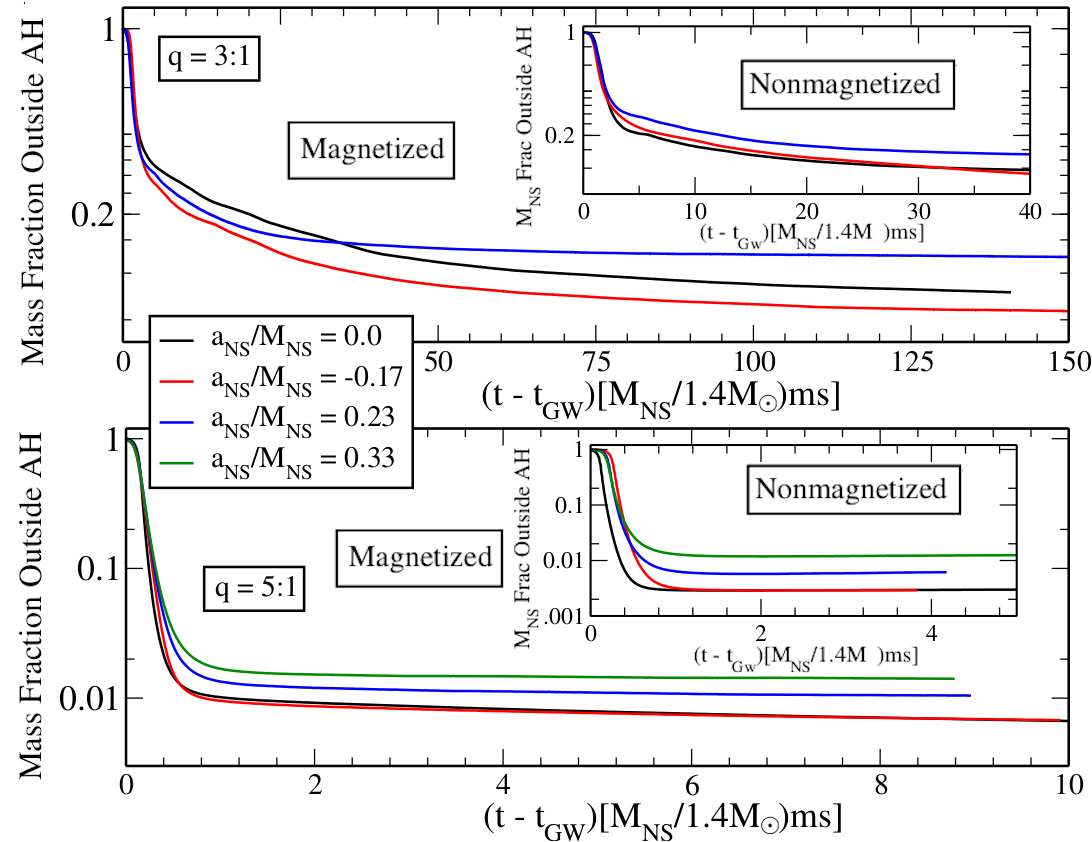
\includegraphics[width=11cm]{rest_mass_fraction}
        \caption[Rest mass outside black hole horizon, as a function of time]{
                    Fraction of rest-mass of the NS outside the apparent horizon of the
                    black hole as a function of coordinate time, for the various
                    configurations considered in \cite{ruiz_2020}. The inset figures
                    report the same for non-magnetized cases, and the coordinate time is
                    shifted such that the merger time coincides with 0.
            }
        \label{fig:rest_mass_fraction}
    \end{figure}

    \begin{figure}[H]
        \centering
        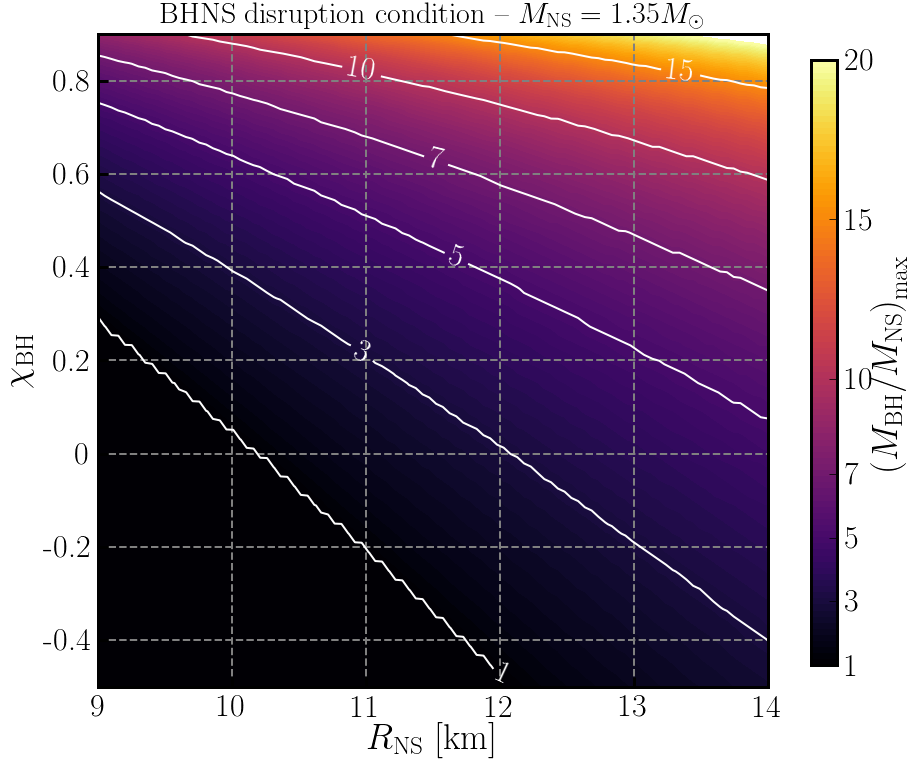
\includegraphics[width=11cm]{nsbh_disruption_condition}
        \caption[Disruption condition in a NSBH binary]{
                    Maximum value of the mass-ratio ($M_{BH}/M_{NS}$) for which a NSBH system
                    disrupts, as a function of the neutron star radius $R_{NS}$, and the aligned
                    component of the dimensionless black hole spin $\chi_{BH}$, assuming $M_{NS} =
                    1.35 M_{\odot}$. Results for other neutron star masses can be obtained by
                    rescaling considering the disruption condition at constant compaction $C_{NS} =
                    GM_{NS}/R_{NS} c^2$. From \cite{foucart_2020}.
            }
        \label{fig:nsbh_disruption_condition}
    \end{figure}
